\title{Error Analysis in PHYS180}
\author{Jordan C. Hanson}
\date{\today}
\documentclass[12pt]{article}
\usepackage[margin=2cm]{geometry}
\usepackage{amsmath,mathtools}
\usepackage{graphicx}

\begin{document}
\maketitle

\begin{abstract}
Scientific measurements cannot be quoted without an assessment of the precision.  We quantify this precision in the form of error analysis.  Rather than originating from \textit{human error}, \textit{statistical errors} arrise from the intrinsic uncertainty encounted in measuring quantities with real instruments.  Further, errors \textit{propagate} through calculations.
\end{abstract}

\section{Instrumental Precision}

The instrumental precision of a piece of data is determined by the smallest division on the instrument.  For example, suppose a length is measured with a meter stick, and the smallest divisions on the meter stick are 1 millimeter.  If the length measured is 31.0 cm, then that result must be stated as $31.0\pm0.1$ cm.

\section{Accuracy versus Precision}

Accuracy and precision are not the same concept.  Accuracy is how far the measured result is from the true value, whereas precision compares the statistical error of a measurement to the measured value itself.  A measurement of $31.0\pm0.1$ cm is precise, because 0.1 cm is small compared to 31.0 cm.  It is not \textit{accurate} if the true length is 29.0 cm.  Why? Because the numbers 31.0 cm and 29.0 cm are separated by $(31.0-29.0)/0.1 = 20$ factors of the error.

\section{Statistical or Random Error}

Suppose a measurement is made with a dial, where a needle is pointing to a number, but vibrating.  When the dial is read one moment, it reads $101.3$ kPa, and in another moment, $101.2$ kPa.  Which pressure measurement of the atmosphere is correct?  It turns out that upon repeated measurements, the \textit{distribution} of measurements resembles Fig. \ref{fig:histo}.

\begin{figure}
\centering
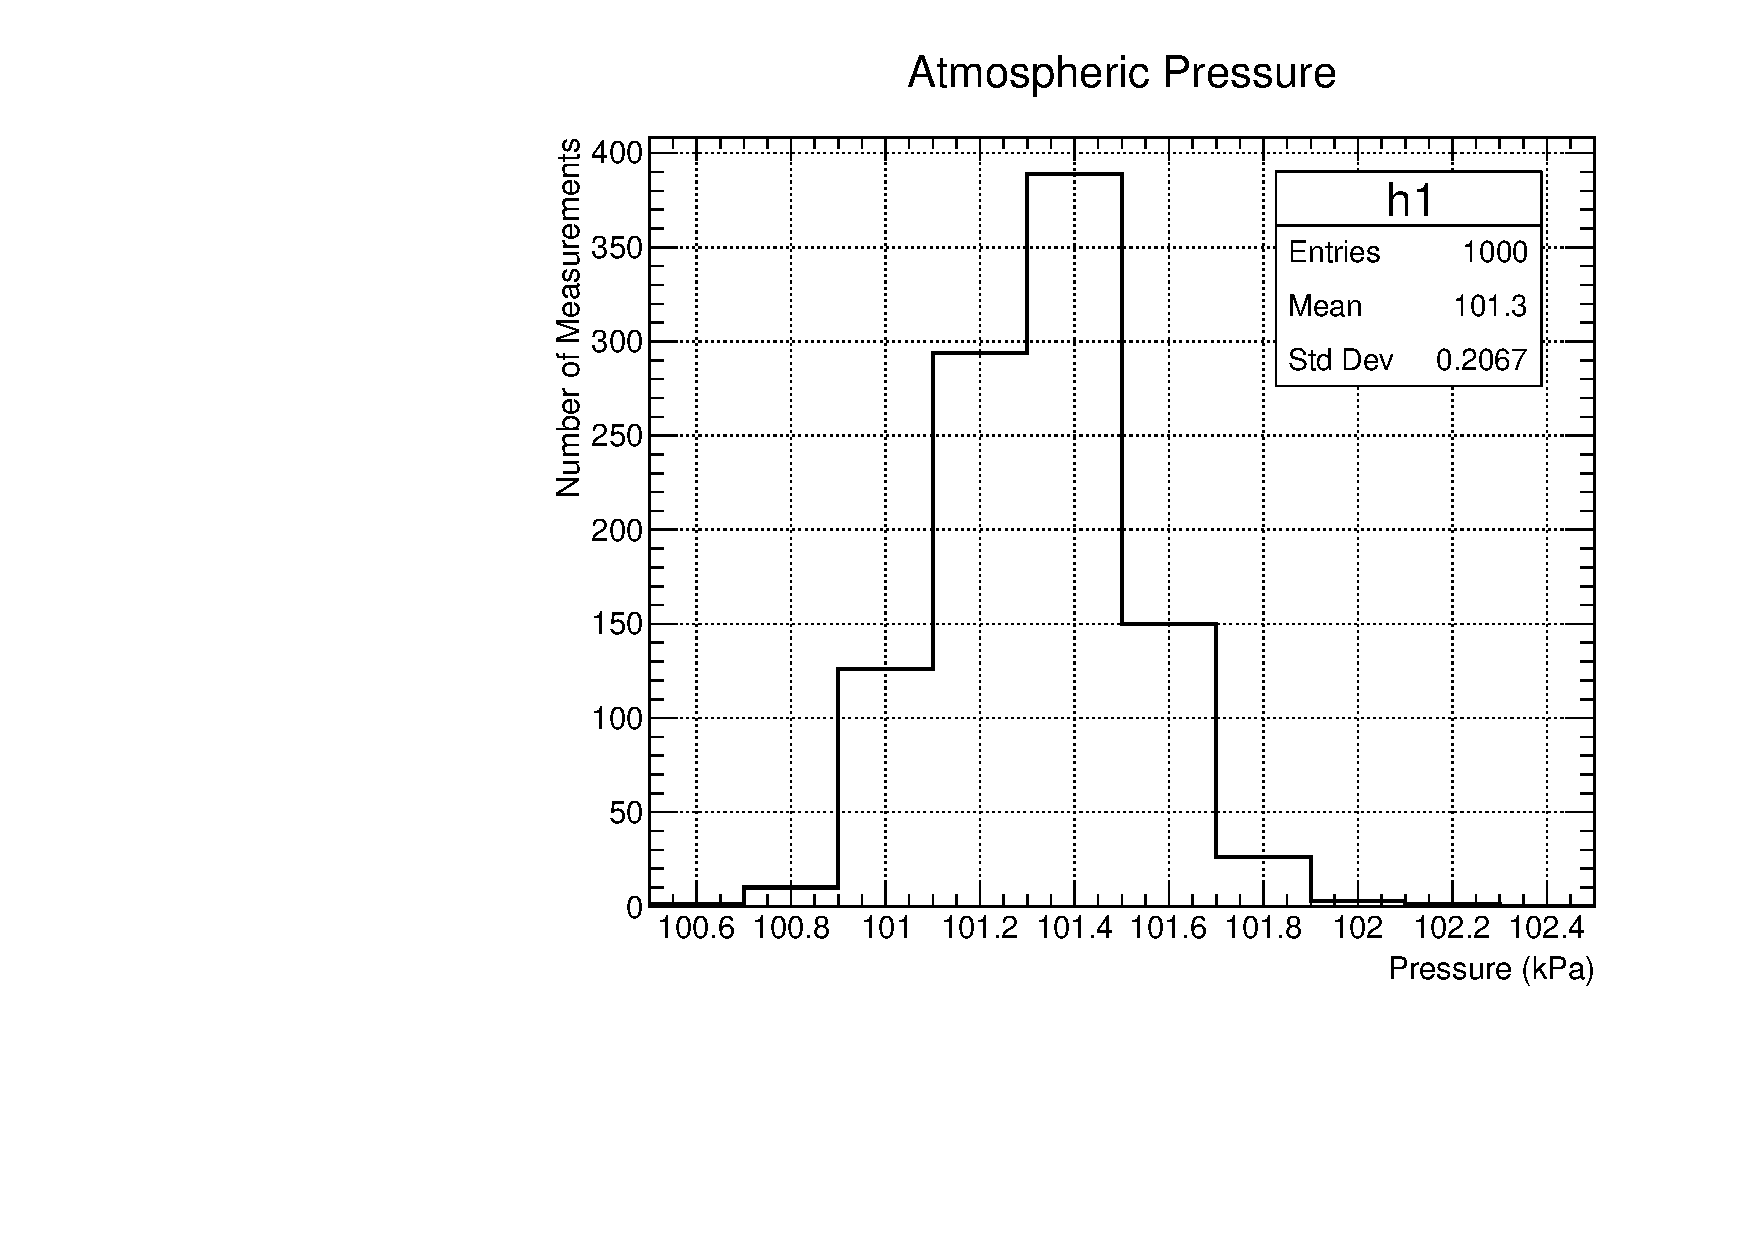
\includegraphics[width=0.5\textwidth]{histo.pdf}
\caption{\label{fig:histo} An example of a distribution of measurements from one instrument: a pressure gauge.}
\end{figure}

The true pressure is most likely 101.3 kPa.  The dial needle is moving, however, making identification of the true pressure impossible.  The true value is ascertained from the statistical distribution.  The \textit{mean} or average of the distribution is 101.3 kPa, and the \textit{standard deviation} is about 0.2 kPa.  Equation \ref{eq:std} represents the standard deviation procedure.  First, the mean $\bar{x}$ is calculated for the collection of measurements $x_i$.  Next, the quantity $(x_i - \bar{x})^2$ is computed for each $x_i$.  Next, the sum of these quantities is found, dividing by $N$\footnote{Technically, we should divide by $N-1$ since the mean has already accounted for one degree of freedom, but in practice where $N$ is a large number, this rarely matters.}, where $N$ is the number of measurements.  This result is called the \textit{variance}, $\sigma^2$.  Finally the square root of the variance is taken to find the standard deviation: $\sqrt{\sigma^2} = \sigma$.

\begin{equation}
\sigma = \sqrt{\frac{1}{N} \left( \sum_{i=1}^N (x_i - \bar{x})^2\right)} \label{eq:std}
\end{equation}

In class, we made measurements of the \textbf{latent heat of fusion} $L_f$ of water.  Those measurements, along with a few more, are listed in Tab. \ref{tab:heat}.  The average latent heat is $340\pm 50$ kJ/kg.  We quote the mean, plus or minus the standard deviation as a sign of the precision of our measurement. 

\begin{table}
\centering
\begin{tabular}{c}
$L_f$ (kJ/kg) \\ \hline
310 \\
389 \\
267 \\
385 \\
319 \\
402 \\
322 \\
341
\end{tabular}
\caption{\label{tab:heat} Some measurements of the laten heat of fusion.  The average is 340 kJ/kg, and the standard deviation is 50 kJ/kg.}
\end{table}

\section{Analysis of Data Subject to Random Error}

\subsection{Addition and Subtraction of variables with errors}

It turns out that computing the mean and standard deviation of a list of results is a different statistical question than assessing the error in a measurement when that measurement is a combination of other measurements.  We measured the latent heat of water by measuring the initial masses and initial temperatures of hot water and ice, and a final temperature of the mixture.  The relevant equation is

\begin{equation}
L_{f,H2O} = c_{H2O} \left( \frac{m_{H20}}{m_{ice}} (T_{i,H20} - T_f) - T_f \right) \label{eq:L}
\end{equation}

The coefficient $c_{H20}$ is the specific heat of water, $m_{ice}$ is the ice mass, $m_{H20}$ is the water mass, $T_{i,H20}$ is the temperature of the hot water, and $T_f$ is the final mixture temperature.  In Tab. \ref{tab:heat}, the mean and the standard deviation represent the average value of the measurements obtained by the class, and the scatter or spread in those measurements.  This is different than assessing the error in \textit{each measurement of $L_f$.}  We saw that the mass measurements were highly precise, maybe $0.5$ grams of error.  Let's ignore errors associated with mass.

What happens to the error in Eq. \ref{eq:L} if we begin to think about errors in temperature?  Notice that two temperatures are subtracted, then multiplied by a mass ratio, and then another temperature is subtracted.  As an example, let's suppose a group used hot water with $T_{i,H20} = 80\pm 2$ $^{\circ}$C, and equal masses of ice and water, and observes a final temperature of $T_f\pm 2$ $^{\circ}$C.  Working in the units of calories, grams, and degrees Celsius, Eq. \ref{eq:L} reduces to

\begin{equation}
L_{f,H20} = \left( T_{i,H20} - 2T_f\right)~~\frac{cal}{g} \label{eq:L2}
\end{equation}

Notice that the group decided that their measurements of temperature were accurate to only about two degrees.  There are two operations happening to temperature in Eq. \ref{eq:L2}.  Multiplication by two, and subtracting two temperatures.  If a variable x has an error $\sigma_x$ associated with it, and it is multiplied by two, the result is

\begin{equation}
2(x\pm \sigma_x) = 2x \pm 2\sigma
\end{equation}

In other words, the error doubles.  In general, for some constant $k$,

\begin{equation}
k(x\pm \sigma_x) = kx \pm k\sigma_x
\end{equation}

Regarding addition and subtraction of variables $x\pm \sigma_x$ and $y\pm \sigma_y$, it turns out that

\begin{align}
(x\pm \sigma_x) + (y\pm \sigma_y) &= (x+y) \pm \sqrt{\sigma_x^2 + \sigma_y^2} \\
(x\pm \sigma_x) - (y\pm \sigma_y) &= (x-y) \pm \sqrt{\sigma_x^2 + \sigma_y^2}
\end{align}

Applying these rules to Eq. \ref{eq:L2} to account for errors yields

\begin{equation}
L_{f,H20} = \left( T_{i,H20} - 2T_f\right) \pm \sqrt{\sigma_{i,H20}^2 + (2\sigma_f)^2}~~\frac{cal}{g} \label{eq:L3}
\end{equation}

The group used two degrees for the error in the initial and final temperatures in Eq. \ref{eq:L3}, and 80 degrees and 0 degrees were the observations.  \textbf{Plugging this information into Eq. \ref{eq:L3} yields} $80 \pm 4.5$ calories per gram.  The expected value is 80 calorie per gram, and the error is $4/80 = 5\%$ of the result.  Dividing the \textit{standard deviation by the result is called the fractional error}.  In the next lesson on error analysis, we will learn to account for multiplication and division of variables through the use of fractional errors.

\subsection{Addition and Subtraction of variables with errors}

If two variables are multiplied or divided, the \textit{fractional errors} are combined rather than the \textit{absolute errors.}  Suppose we are trying to quantify the momentum of a system with mass $m$ and speed $v$:

\begin{equation}
p = mv
\end{equation}

We measure the mass: $m\pm \sigma_m$, and the speed: $v\pm\sigma_v$.  The \textit{fractional error} in the momentum, speed, and mass are $\frac{\sigma_p}{p}$, $\frac{\sigma_v}{v}$, and $\frac{\sigma_m}{m}$ respectively.  The relationship between the fractional error in momentum and the other two is

\begin{equation}
\left(\frac{\sigma_p}{p}\right)^2 = \left(\frac{\sigma_m}{m}\right)^2 + \left(\frac{\sigma_v}{v}\right)^2
\end{equation}

Notice that the fractional errors of the mass and speed are added in quadrature (summing squares) to produce the frational error of the momentum.  Thus, to quote a measurement of momentum, the result is:

\begin{equation}
p = (mv) \pm (mv) \sqrt{\left(\frac{\sigma_m}{m}\right)^2 + \left(\frac{\sigma_v}{v}\right)^2}
\end{equation}

\end{document}